
\begin{figure}
    \centering
    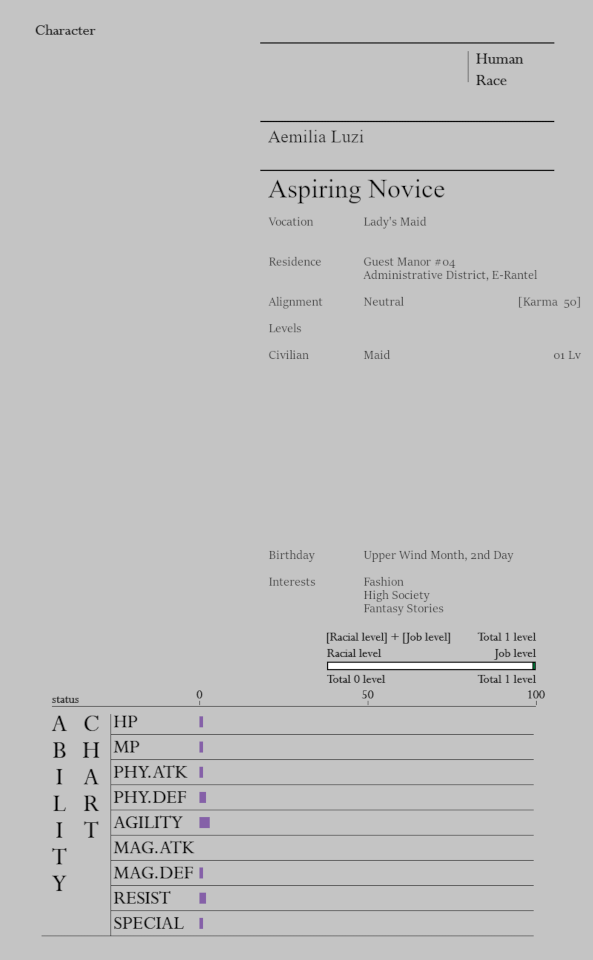
\includegraphics[width=1\linewidth]{V1 Birthright//images/NaUEKrB.png}
    \caption*{Aemilia Luzi Character Sheet}
\end{figure}

\section*{The Noble Household (Part I)}

The noble household employs a myriad of servants and retainers: from iconic Butlers and Maids, to Men-at-Arms, Cooks, Groundskeepers and Pages(to name a few). These individuals that serve the aristocratic estate are far from the shallow imitations that occasionally appear to work on an intermittent basis, functioning as some part of common hospitality to create a transient atmosphere of wealth and luxury. Members of a noble household are retainers which often serve as close personal attendants of noble families in all matters mundane.

 

In a world where fending for oneself often entails risk of debilitating injury, death or worse, a stable life in honoured service under the protection of a powerful family is an enticing prospect for those without the means to make their own way – or those confident that their skills in stewardship can be put to use leveraging the wealth and influence of a noble master.

 

Yet as menial as the lowest of these positions may seem, those with hopeful prospects must pass stringent filters; only those who are deemed suitable will be invited to assume the positions of trust that expose one to the inner workings of a noble house and the private lives of their families. Freedmen may enter into the lowest ranks of household hierarchy, while those of noble blood may start in roles that suit their education and upbringing. However, only those possessed of experience and talent usually rise to the highest positions of authority.

 

A noble's household may be seen as the family of vassals that most closely surrounds the family that they serve. While individually not as prominent as their Lords and Ladies, they are collectively the most visible aspect of a Noble House. They carry within them the honor, will and pride of their houses, representing them in the many aspects of daily life in a demesne.

 

Vampiric Households are a dark mirror of the noble household: bound to their master – willingly or unwillingly – in eternal undead servitude.



\chapter{Ludmila Zahradnik}

Ludmila hummed to herself whilst sitting in front of the large dresser mirror, slowly brushing out her hair with an old, reliable lacquered comb that had been in her possession since she was a girl. She wasn’t in a bad mood before, but the hot bath had put her into a much better one as surely as soaking in the warm water had lent the sensation of melting away the day’s stress and worries. Knowing that Lady Shalltear was already willing to assist her efforts to restore Warden’s Vale lightened the burdens weighing on her mind, and she now focused her thoughts on how one might best address the problems that she had seen and heard described in E-Rantel.

 

One of the maids brought in by Yuri Alpha hovered nervously somewhere to her side, holding a spare towel, while another was preparing her outfit for dinner. Judging by the sounds coming from below, there seemed to be a few others working around the manor. She glanced at the reflection of the maid waiting on her – it seemed like she had put at least some effort into maintaining her haggard appearance, but it felt mostly the same as the other residents that she had seen so far. The women were tired and frightened: long days in such a state had left them in a nervous and jumpy condition. When one of the Undead sentries provided by Yuri Alpha came stomping in with two barrels of steaming hot water, the both of them screamed and fled to cower in the furthest corner of the solar and stayed there. Ludmila ended up having the unique experience of instructing a Death Knight on how to draw a bath.

 

It was a long while after it had stomped back out of the room that the pair came out of hiding, and by then Ludmila was already half done on her own. Beyond that, the maids seemed very new at their jobs. In previous years, the city had similarly provided maids for visiting nobles who rented the guest houses and the current maids seemed to be quite unpracticed by comparison. Their movements seemed stiff and unsure; they seem to be constantly second guessing themselves as they worked. It was to the point that their insecurity was subtly affecting those around them, and Ludmila frowned as she had to mentally wave the feeling away. As Yuri Alpha had demonstrated earlier in the evening, confidence and form inspired the same in those around her, and so it seemed that the reverse was true as well.

 

Ludmila thought back to Vilette Jezne and her actions during the gathering of nobles. Perhaps her haranguing of the others was a different facet of the same idea: to provoke a sense of normalcy and routine that caused others to act out of habit. While she had no aspiration to become a crotchety old crab, Ludmila thought she might be able to achieve those same results in her own way. And so, she simply went about her preparations for dinner, methodically running down a mental checklist of her own routines as she moved about the room in her ongoing preparations. It did not take long until the two maids also started to move, trying to keep up with and eventually anticipating her actions. These maids had obviously undergone some sort of training, but they probably had no opportunity to put their training to work with the state of E-Rantel as it was.

 

She stood and waited in a fresh linen shift as the maids brought her dress to her. Though the hearth had been stocked and lit, the air in the room was still warming up. She suppressed a shiver as she mentally willed the maids to move faster. The dress had been purchased last winter, as a reward for her own hard work helping to organize the Barony that year. It was something she thought might suit both their brief appearances in E-Rantel as well as the few festive events at home. It had a pleated white cotton blouse, with long sleeves and black buttons which ran up and under the ruffled bow tie which spilled from the collar. A wide kidney belt fashioned from leather wrapped over the waist, separating the blouse from the long, three panel skirt made from linen dyed in forest green. An open bolero matched the skirt, decorated with buttons between the elbow and wrist. The dress was warm enough for winter in E-Rantel, and she only needed to wear a coat over it to be serviceable in the highlands.

 

It had been on display in the window of a boutique near the main plaza, and she spotted it while her family was on the way back from selling their goods at the various merchant warehouses in the outskirts – she immediately hopped off their moving wagon and bought it with over half of her earnings for the year. After she returned triumphantly with her spoils, her brothers had wailed upon hearing the cost of the entire outfit, as it was enough to buy half a suit of masterwork plate armour. Her father just seemed relieved that his only daughter was not just a tomboy after years of being raised in a household full of men.

 

As she was now helped into the dress by her maids, however, a vague sense of annoyance filled her as she saw that her ambitions of yesteryear had been somewhat misplaced. She had grown taller, causing the hem of her skirt to come two thirds of the way up to her knee. The pleated blouse did not fill out as much as she had hoped that it would, leaving it loose over her chest. Ludmila resisted the urge to sigh as the maids fussed over her appearance. When they were nearly finished, one finally spoke.

 

“Frontier Nobles really are amazing…”

 

Aemilia Luzi was the younger of the two maids, who had arrived and introduced themselves just before the Death Knight had come to deliver water for the bath. The girl was half a head shorter than Ludmila, with shoulder-length auburn hair and a face full of light freckles. Her emerald eyes glimmered as she continued.

 

“Even in a beautiful dress, you look like a gallant warrior at the same time. Everything about it suits you so well while making it seem like you could go to battle just like that. Even the hem of your skirt is raised so you can move around easily, when other ladies might have chosen a more reserved appearance.”

 

The excited maid made a motion with her right arm, as if she was swinging a sword, or perhaps clubbing someone with a rolling pin...or stabbing something with a fork? Ludmila could not tell.

 

“...how do you do it, my lady?” She asked.

 

Aemilia’s voice lost its excited tinge, turning subdued. Ludmila looked down at her dress, searching for any problems with the outfit. She didn’t notice anything wrong in the mirror, either.

 

“Do what?”

 

The maid’s work slowed, until her hands stopped moving entirely. She looked up to Ludmila with an expression that was a mixture of awe and uncertainty.

 

“How do you live your life like everything is normal?” She said, “I’ve heard some others talk about how they saw you walking outside this evening, all by yourself in the noble’s district like it was just a regular spring day. I thought that maybe that was an exaggerated rumor, but then that monster came into the room just now and you just continued on like nothing at all was strange.”

 

Ludmila opened her mouth, then closed it again, uncertain how to respond. She didn’t feel like she had done anything that anyone else couldn’t have. It wasn’t as if she never panicked, or did not feel fear or insecurity. Even her actions around the maids were just an experiment that she was not even sure would work or not, inspired by what she had experienced previously that day. She thought that a straightforward answer would be best.

 

“I don’t think I’ve done anything special,” she said, “and this is hardly normal for me. I was frightened at first, when I saw all of the Undead in the city, but then I realized that fear for its own sake was unreasonable. I simply decided that I had more important things to do; that I could not afford a life that had me jumping at every shadow. That the days and seasons would pass; that the world would continue to run outside of our borders. That in spite of all of my fears and uncertainty, I still needed to fulfil my duties to the land or my fief would fall to ruin.”

 

Aemilia’s eyes were sparkling again, but a dismissive sniff from Ludmila’s other arm indicated that the second maid did not see things the same way. Terah Ro'eh’s husky voice was about as incredulous as one could get without sounding outright disrespectful.

 

“You decided?” She said, “My lady, if we could all just get up one morning and decide to get back to life as usual, no one would be hiding in their homes now, would they?”

 

“She’s right,” Aemilia said reluctantly, “even the other nobles tried a day or two ago. A few of the ladies riled up one of the boys to show them how brave they were, so he marched out of the clubhouse with everyone following a safe distance away. He stormed right up to one of those Death Knights and soiled himself as soon as he came within a few strides, collapsing on the ground in a puddle. When the Undead monster turned to look our way, everyone screamed and ran all the way back to the clubhouse, leaving the poor nobleman lying on the street.”

 

Terah nodded at the other maid’s words, her black curls bouncing over the dusky skin of her cheeks.

 

“That’s right,” she said. “In the end, Miss Alpha had to carry him back to his manor. The poor kid was out cold. Mark my words: Frontier Nobles are made different, somehow. When times are good those other nobles might know how to boss people around, but all the boasting and bragging and talk of being brave captains and fierce fighters is like it never was when it comes down to it.”

 

Her attendant’s disdain for the rest of the nobility was alarming, to say the least. Ludmila felt a tugging obligation to at least salvage at least a little bit of her peers’ respect.

 

“Then what about Yuri Alpha?” Ludmila asked, “She doesn’t seem to mind everything that goes on. If anything, she seems to carry herself far better than I do.”

 

“You’re right, my lady,” Aemilia replied, “but...she’s one of the Royal Maids, you know? She’s probably had a long time getting used to all that, or maybe she’s not what she seems to be at all.”

 

Ludmila thought Yuri Alpha did not appear to be abnormal in any way, so she decided to follow up on the first idea.

 

“Then maybe all it takes is time,” she suggested. “The two of you seem to be gossiping quite bravely here, after all.”

 

The animated atmosphere instantly turned solemn as the two maids exchanged glances. Terah was the first to recover, glancing at Ludmila as she spoke.

 

“A little time then, my lady?” Terah said, “Maybe you’re right, but you still won’t catch me walking up to those Undead any time soon.”

 

“You...you won’t tell anyone about what we said before, will you, my lady?” Aemilia asked.

 

“Not this time, no,” Ludmila answered. “In the future, however, I will not defend you with falsehoods if you are caught slandering the Royal Household or His Majesty’s nobility.”

 

The two maids stood and stepped back, having completed her outfit. They curtseyed in unison as Ludmila stepped off of the dressing stool and headed out of the solar.

 

“Thank you, Lady Zahradnik.”